\documentclass[11pt,a4paper]{report}
\usepackage[textwidth=37em,vmargin=30mm]{geometry}
\usepackage{calc,xunicode,amsmath,amssymb,paralist,enumitem,tabu,booktabs,datetime2,xeCJK,xeCJKfntef,listings}
\usepackage{tocloft,fancyhdr,tcolorbox,xcolor,graphicx,eso-pic,xltxtra,xelatexemoji}

\newcommand{\envyear}[0]{2025}
\newcommand{\envdatestr}[0]{2025-09-25}
\newcommand{\envfinaldir}[0]{webdb/2025/20250925/final}

\usepackage[hidelinks]{hyperref}
\hypersetup{
    colorlinks=false,
    pdfpagemode=FullScreen,
    pdftitle={Web Digest - \envdatestr}
}

\setlength{\cftbeforechapskip}{10pt}
\renewcommand{\cftchapfont}{\rmfamily\bfseries\large\raggedright}
\setlength{\cftbeforesecskip}{2pt}
\renewcommand{\cftsecfont}{\sffamily\small\raggedright}

\setdefaultleftmargin{2em}{2em}{1em}{1em}{1em}{1em}

\usepackage{xeCJK,xeCJKfntef}
\xeCJKsetup{PunctStyle=plain,RubberPunctSkip=false,CJKglue=\strut\hskip 0pt plus 0.1em minus 0.05em,CJKecglue=\strut\hskip 0.22em plus 0.2em}
\XeTeXlinebreaklocale "zh"
\XeTeXlinebreakskip = 0pt


\setmainfont{Brygada 1918}
\setromanfont{Brygada 1918}
\setsansfont{IBM Plex Sans}
\setmonofont{JetBrains Mono NL}
\setCJKmainfont{Noto Serif CJK SC}
\setCJKromanfont{Noto Serif CJK SC}
\setCJKsansfont{Noto Sans CJK SC}
\setCJKmonofont{Noto Sans CJK SC}

\setlength{\parindent}{0pt}
\setlength{\parskip}{8pt}
\linespread{1.15}

\lstset{
	basicstyle=\ttfamily\footnotesize,
	numbersep=5pt,
	backgroundcolor=\color{black!5},
	showspaces=false,
	showstringspaces=false,
	showtabs=false,
	tabsize=2,
	captionpos=b,
	breaklines=true,
	breakatwhitespace=true,
	breakautoindent=true,
	linewidth=\textwidth
}






\newcommand{\coverpic}[2]{
    % argv: itemurl, authorname
    Cover photo by #2~~(\href{#1}{#1})
}
\newcommand{\makeheader}[0]{
    \begin{titlepage}
        % \newgeometry{hmargin=15mm,tmargin=21mm,bmargin=12mm}
        \begin{center}
            
            \rmfamily\scshape
            \fontspec{BaskervilleF}
            \fontspec{Old Standard}
            \fontsize{59pt}{70pt}\selectfont
            WEB\hfill DIGEST
            
            \vfill
            % \vskip 30pt
            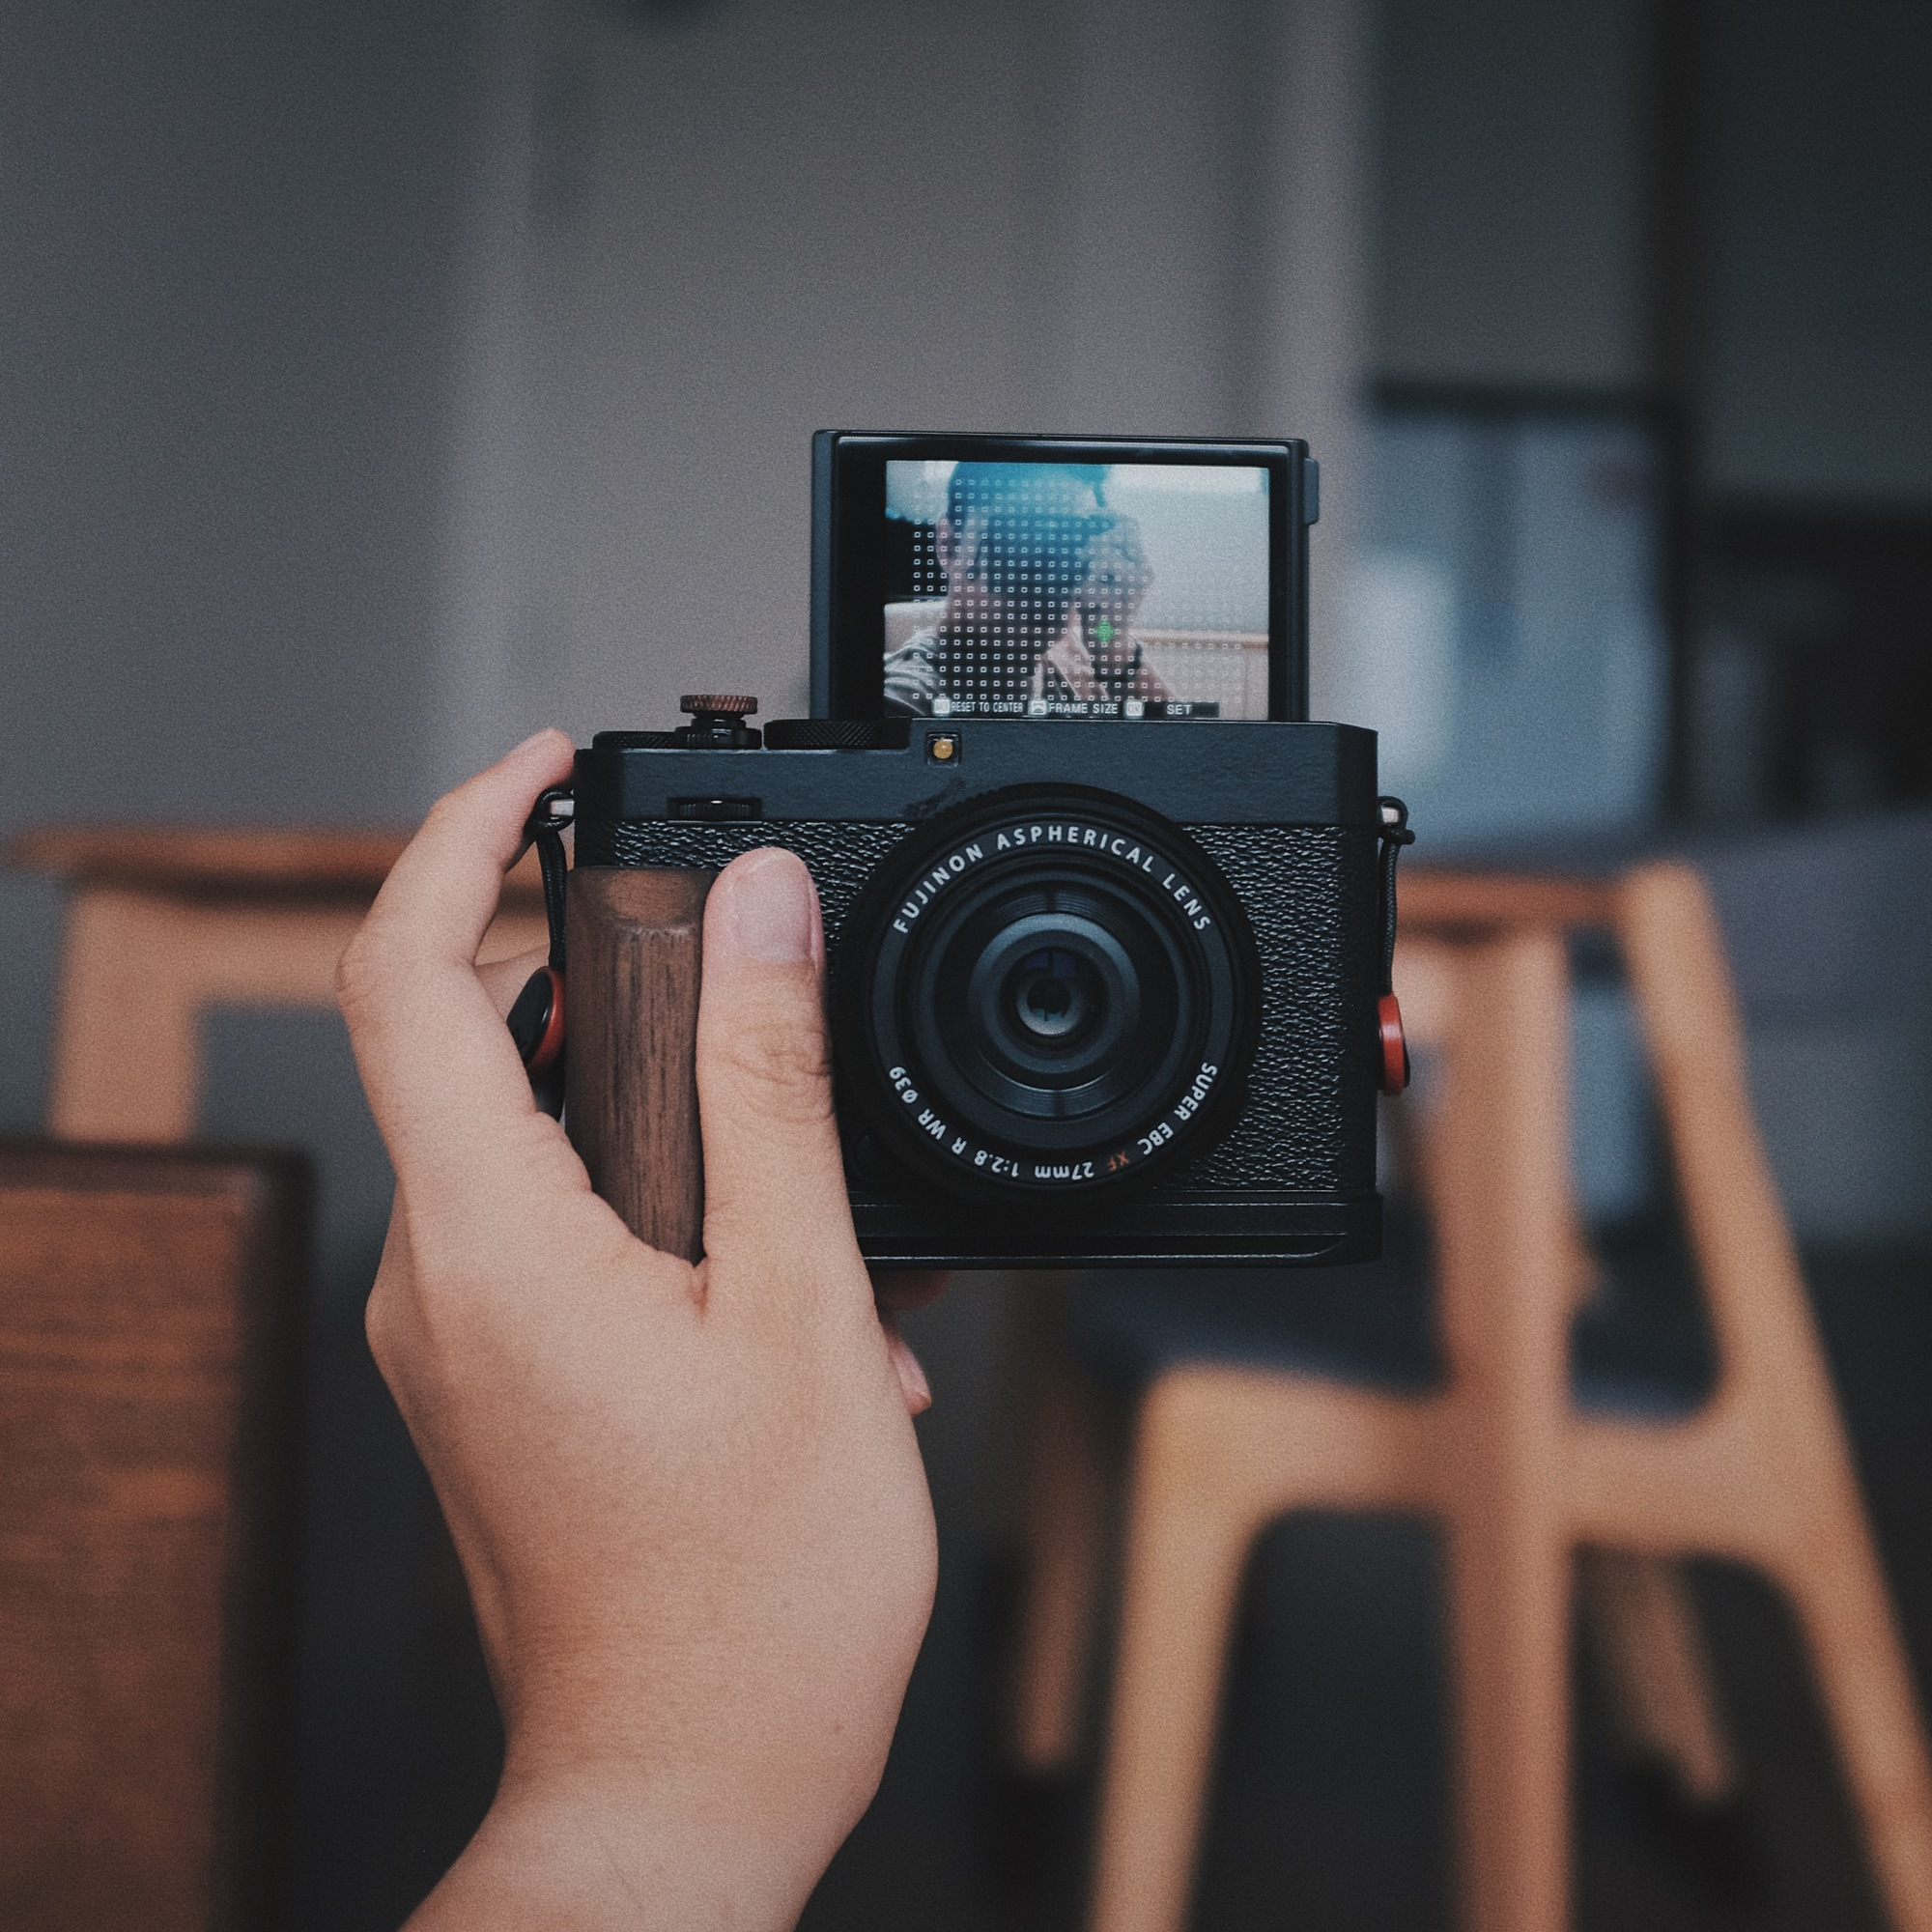
\includegraphics[width=\linewidth]{\envfinaldir/coverpic-prod.jpg}\par
            % \vskip 30pt
            \vfill

            \normalsize\rmfamily\scshape
            \copyright{} The Web Digest Project \hfill\large \envdatestr
        \end{center}
    \end{titlepage}
    % \restoregeometry
}
\newcommand{\simplehref}[1]{%
    \textcolor{blue!80!green}{\href{#1}{#1}}%
}
\renewcommand{\contentsname}{\center\Huge\sffamily\bfseries Contents\par\vskip 20pt}
\newcounter{ipartcounter}
\setcounter{ipartcounter}{0}
\newcommand{\ipart}[1]{
    % \vskip 20pt
    \clearpage
    \stepcounter{ipartcounter}
    \phantomsection
    \addcontentsline{toc}{chapter}{#1}
    % \begin{center}
    %     \Huge
    %     \sffamily\bfseries
    %     #1
    % \end{center}
    % \vskip 20pt plus 7pt
}
\newcounter{ichaptercounter}
\setcounter{ichaptercounter}{0}
\newcommand{\ichapter}[1]{
    % \vskip 20pt
    \clearpage
    \stepcounter{ichaptercounter}
    \phantomsection
    \addcontentsline{toc}{section}{\numberline{\arabic{ichaptercounter}}#1}
    \begin{center}
        \Huge
        \sffamily\bfseries
        #1
    \end{center}
    \vskip 20pt plus 7pt
}
\newcommand{\entrytitlefont}[1]{\subsection*{\raggedright\Large\sffamily\bfseries#1}}
\newcommand{\entryitemGeneric}[2]{
    % argv: title, url
    \parbox{\linewidth}{
        \entrytitlefont{#1}\par\vskip 5pt
        \footnotesize\ttfamily\mdseries
        \simplehref{#2}
    }\vskip 11pt plus 11pt minus 1pt
}
\newcommand{\entryitemGithub}[3]{
    % argv: title, url, desc
    \parbox{\linewidth}{
        \entrytitlefont{#1}\par\vskip 5pt
        \footnotesize\ttfamily\mdseries
        \simplehref{#2}\par\vskip 5pt
        \small\rmfamily\mdseries#3
    }\vskip 11pt plus 11pt minus 1pt
}
\newcommand{\entryitemAp}[3]{
    % argv: title, url, desc
    \parbox{\linewidth}{
        \entrytitlefont{#1}\par\vskip 5pt
        \footnotesize\ttfamily\mdseries
        \simplehref{#2}\par\vskip 5pt
        \small\rmfamily\mdseries#3
    }\vskip 11pt plus 11pt minus 1pt
}
\newcommand{\entryitemHackernews}[3]{
    % argv: title, hnurl, rawurl
    % \parbox{\linewidth}{
    %     \entrytitlefont{#1}\par\vskip 5pt
    %     \footnotesize\ttfamily\mdseries
    %     \simplehref{#3}\par
    %     \textcolor{black!50}{\href{#2}{#2}}
    % }\vskip 11pt plus 11pt minus 1pt
    \begin{minipage}{\linewidth}
            \entrytitlefont{#1}\par\vskip 5pt
            \footnotesize\ttfamily\mdseries
            \simplehref{#3}\par
            \textcolor{black!50}{\href{#2}{#2}}
    \end{minipage}\par\vskip 11pt plus 11pt minus 1pt
}







\begin{document}

\makeheader

\tableofcontents\clearpage




\ipart{Developers}
\ichapter{Hacker News}
\entryitemTwoLinks{Everything that's wrong with Google Search in one image}{https://news.ycombinator.com/item?id=45366566}{https://bitbytebit.substack.com/p/everything-thats-wrong-with-google}

\entryitemTwoLinks{Tinder, Hinge, and their corporate owner keep rape under wraps}{https://news.ycombinator.com/item?id=45363429}{https://themarkup.org/investigations/2025/02/13/dating-app-tinder-hinge-cover-up}

\entryitemTwoLinks{Terence Tao: The role of small organizations in society has shrunk significantly}{https://news.ycombinator.com/item?id=45362697}{https://mathstodon.xyz/@tao/115259943398316677}

\entryitemTwoLinks{Product Hunt is dead}{https://news.ycombinator.com/item?id=45362569}{https://sedimental.org/product\_hunt\_is\_dead.html}

\entryitemTwoLinks{Zed's Pricing Has Changed: LLM Usage Is Now Token-Based}{https://news.ycombinator.com/item?id=45362425}{https://zed.dev/blog/pricing-change-llm-usage-is-now-token-based}

\entryitemTwoLinks{New bacteria, and two potential antibiotics, discovered in soil}{https://news.ycombinator.com/item?id=45362254}{https://www.rockefeller.edu/news/38239-hundreds-of-new-bacteria-and-two-potential-antibiotics-found-in-soil/}

\entryitemTwoLinks{SedonaDB: A new geospatial DataFrame library written in Rust}{https://news.ycombinator.com/item?id=45362206}{https://sedona.apache.org/latest/blog/2025/09/24/introducing-sedonadb-a-single-node-analytical-database-engine-with-geospatial-as-a-first-class-citizen/}

\entryitemTwoLinks{Python on the Edge: Fast, sandboxed, and powered by WebAssembly}{https://news.ycombinator.com/item?id=45362023}{https://wasmer.io/posts/python-on-the-edge-powered-by-webassembly}

\entryitemTwoLinks{How to be a leader when the vibes are off}{https://news.ycombinator.com/item?id=45361394}{https://chaoticgood.management/how-to-be-a-leader-when-the-vibes-are-off/}

\entryitemTwoLinks{The DHS has been harvesting DNA from Americans for years}{https://news.ycombinator.com/item?id=45361239}{https://www.wired.com/story/dhs-has-been-collecting-us-citizens-dna-for-years/}

\entryitemTwoLinks{Just let me select text}{https://news.ycombinator.com/item?id=45360475}{https://aartaka.me/select-text.html}

\entryitemTwoLinks{How to Lead in a Room Full of Experts}{https://news.ycombinator.com/item?id=45359604}{https://idiallo.com/blog/how-to-lead-in-a-room-full-of-experts}

\entryitemTwoLinks{Learning Persian with Anki, ChatGPT and YouTube}{https://news.ycombinator.com/item?id=45359524}{https://cjauvin.github.io/posts/learning-persian/}

\entryitemTwoLinks{US airlines are pushing to remove protections for passengers and add more fees}{https://news.ycombinator.com/item?id=45359378}{https://www.travelandtourworld.com/news/article/american-joins-delta-southwest-united-and-other-us-airlines-push-to-strip-away-travelers-rights-and-add-more-fees-by-rolling-back-key-protections-in-new-deregulation-move/}

\entryitemTwoLinks{Rights groups urge UK PM Starmer to abandon plans for mandatory digital ID}{https://news.ycombinator.com/item?id=45359356}{https://bigbrotherwatch.org.uk/press-releases/rights-groups-urge-starmer-to-abandon-plans-for-mandatory-digital-id/}

\entryitemTwoLinks{EU age verification app not planning desktop support}{https://news.ycombinator.com/item?id=45359074}{https://github.com/eu-digital-identity-wallet/av-doc-technical-specification/issues/22}

\entryitemTwoLinks{Yt-dlp: Upcoming new requirements for YouTube downloads}{https://news.ycombinator.com/item?id=45358980}{https://github.com/yt-dlp/yt-dlp/issues/14404}

\entryitemTwoLinks{Huntington's disease treated for first time}{https://news.ycombinator.com/item?id=45358940}{https://www.bbc.com/news/articles/cevz13xkxpro}

\entryitemTwoLinks{My game's server is blocked in Spain whenever there's a football match on}{https://news.ycombinator.com/item?id=45358433}{https://old.reddit.com/r/gamedev/comments/1np6kyn/my\_games\_server\_is\_blocked\_in\_spain\_whenever/}

\entryitemTwoLinks{How AWS S3 serves 1 petabyte per second on top of slow HDDs}{https://news.ycombinator.com/item?id=45358280}{https://bigdata.2minutestreaming.com/p/how-aws-s3-scales-with-tens-of-millions-of-hard-drives}\ichapter{Phoronix}
\entryitemGeneric{\hskip 0pt{}Qualcomm Announces X2 Elite SoCs - Up To 18 Cores \& Up To 5.0GHz Boost Frequency}{https://www.phoronix.com/news/Qualcomm-X2-Elite-Announced}

\entryitemGeneric{\hskip 0pt{}Linux Laptop Vendor MALIBAL Attempting To Pursue Made-In-USA Laptops}{https://www.phoronix.com/news/MALIBAL-Made-In-US-Laptops}

\entryitemGeneric{\hskip 0pt{}The Massive AI Performance Benefit With AMX On Intel Xeon 6 "Granite Rapids"}{https://www.phoronix.com/review/intel-xeon-6-granite-rapids-amx}

\entryitemGeneric{\hskip 0pt{}Mesa's PowerVR Vulkan Driver Gets Rid Of Its Old Hardcoded Shader Code}{https://www.phoronix.com/news/PowerVR-Drops-Hard-Shader-Code}

\entryitemGeneric{\hskip 0pt{}Intel Moves Pre-Arc Graphics To "Legacy" Driver On Windows - Linux Users Need Not Worry}{https://www.phoronix.com/news/Intel-11th-14th-Gen-Legacy-Drv}

\entryitemGeneric{\hskip 0pt{}GCC 16 Will No Longer Treat Function Multi-Versioning As Experimental On ARM64}{https://www.phoronix.com/news/GCC-16-Stable-ARM64-FMV}

\entryitemGeneric{\hskip 0pt{}FFmpeg Introduces MPEG-H 3D Audio Decoding Support}{https://www.phoronix.com/news/FFmpeg-:ands-MPEG-H-3D-Decode}

\entryitemGeneric{\hskip 0pt{}Sony DualSense Controller Audio Jack Handling Ready For Linux 6.18}{https://www.phoronix.com/news/Sony-DualSense-Audio-Handling}

\entryitemGeneric{\hskip 0pt{}SquashFS Optimization Achieves 15,277x Performance In Developer Benchmark}{https://www.phoronix.com/news/SquashFS-Faster-Sparse-Copy}


\ipart{Developers~~~~(zh-Hans)}
\ichapter{Solidot}
\entryitemGeneric{\hskip 0pt{}YouTube 放弃事实核查政策}{https://www.solidot.org/story?sid=82400}

\entryitemGeneric{\hskip 0pt{}越南因生物识别规则关闭数百万银行账号}{https://www.solidot.org/story?sid=82399}

\entryitemGeneric{\hskip 0pt{}加州律师因 ChatGPT 伪造案例被罚款 1 万美元}{https://www.solidot.org/story?sid=82398}

\entryitemGeneric{\hskip 0pt{}人的大部分行为是出于习惯}{https://www.solidot.org/story?sid=82397}

\entryitemGeneric{\hskip 0pt{}伊朗程序员的西方 IT 服务使用经历}{https://www.solidot.org/story?sid=82396}

\entryitemGeneric{\hskip 0pt{}多地推进采集男性居民血样}{https://www.solidot.org/story?sid=82395}

\entryitemGeneric{\hskip 0pt{}BMI 指数过低死亡风险可能更高}{https://www.solidot.org/story?sid=82394}

\entryitemGeneric{\hskip 0pt{}TikTok 算法将在美国重新训练}{https://www.solidot.org/story?sid=82393}

\entryitemGeneric{\hskip 0pt{}Google TV 加入 Gemini AI 助手}{https://www.solidot.org/story?sid=82392}

\entryitemGeneric{\hskip 0pt{}Windows 11 支持将视频设为墙纸}{https://www.solidot.org/story?sid=82390}

\entryitemGeneric{\hskip 0pt{}英伟达向 OpenAI 投资千亿美元}{https://www.solidot.org/story?sid=82389}

\entryitemGeneric{\hskip 0pt{}埃及总统赦免 Alaa Abdel Fattah}{https://www.solidot.org/story?sid=82388}

\entryitemGeneric{\hskip 0pt{}Multi-Kernel 架构支持代码公开}{https://www.solidot.org/story?sid=82386}

\entryitemGeneric{\hskip 0pt{}Tails 7.0 释出}{https://www.solidot.org/story?sid=82385}

\entryitemGeneric{\hskip 0pt{}BlockBlasters 游戏补丁被发现含有恶意程序}{https://www.solidot.org/story?sid=82384}

\entryitemGeneric{\hskip 0pt{}中国海军成功测试舰载机电磁弹射}{https://www.solidot.org/story?sid=82383}

\entryitemGeneric{\hskip 0pt{}英国银行仍然运行 1960 年代写的代码}{https://www.solidot.org/story?sid=82382}

\entryitemGeneric{\hskip 0pt{}西雅图艰难应对科技工作减少}{https://www.solidot.org/story?sid=82381}

\entryitemGeneric{\hskip 0pt{}天文学家在地球附近发现一颗准卫星}{https://www.solidot.org/story?sid=82380}

\entryitemGeneric{\hskip 0pt{}微软的 Entra ID 漏洞可能造成灾难性的后果}{https://www.solidot.org/story?sid=82379}\ichapter{V2EX}
\entryitemGeneric{\hskip 0pt{}[问与答] 像我这种塞尔达打人马都费劲的玩家适合《艾尔登法环》么?}{https://www.v2ex.com/t/1161654}

\entryitemGeneric{\hskip 0pt{}[分享发现] [征友链] 网站恢复运营,寻找友情链接}{https://www.v2ex.com/t/1161653}

\entryitemGeneric{\hskip 0pt{}[分享发现] T-Mobile 转 PayGo+靓号 Port in}{https://www.v2ex.com/t/1161652}

\entryitemGeneric{\hskip 0pt{}[问与答] 请教两个词语}{https://www.v2ex.com/t/1161651}

\entryitemGeneric{\hskip 0pt{}[宽带症候群] 上海宽带咨询~~~~}{https://www.v2ex.com/t/1161649}

\entryitemGeneric{\hskip 0pt{}[宽带症候群] 想问下上海链家省心租赠送的电信宽带能否自行改桥接}{https://www.v2ex.com/t/1161648}

\entryitemGeneric{\hskip 0pt{}[分享发现] 应用宝 PC 版登录微信,被风险了}{https://www.v2ex.com/t/1161646}

\entryitemGeneric{\hskip 0pt{}[分享创造] 开发了一个为程序员设计的项目管理软件}{https://www.v2ex.com/t/1161644}

\entryitemGeneric{\hskip 0pt{}[推广] 免信用卡订阅 ChatGPT plus,一站式 APP 内购服务平台自荐}{https://www.v2ex.com/t/1161642}

\entryitemGeneric{\hskip 0pt{}[Nintendo Switch] 有没有 switch 卡带平台推荐}{https://www.v2ex.com/t/1161641}

\entryitemGeneric{\hskip 0pt{}[分享创造] 一个纯前端运行的 Markdown 转 PDF 小工具}{https://www.v2ex.com/t/1161640}

\entryitemGeneric{\hskip 0pt{}[推广] 阿里刚放出的 Wan2.5(通义万相 2.5 Preview),升级点很硬}{https://www.v2ex.com/t/1161639}

\entryitemGeneric{\hskip 0pt{}[问与答] 苹果的跨设备复制粘贴经常实效(mbp 和 mac mini)求替代品}{https://www.v2ex.com/t/1161638}

\entryitemGeneric{\hskip 0pt{}[Linux] Debian 13 的 Gnome 48 似乎有点 bug,换成 Fedora 就没事。试用了一段时间,我原以为 Gnome 默认 Dark Mode,没想到还能更加 Dark}{https://www.v2ex.com/t/1161637}

\entryitemGeneric{\hskip 0pt{}[Bitcoin] 悬赏:有人了解门头沟赔偿的后续进展吗?}{https://www.v2ex.com/t/1161636}

\entryitemGeneric{\hskip 0pt{}[VXNA] 申请收录个人博客: https://blog.tjdata.site}{https://www.v2ex.com/t/1161635}

\entryitemGeneric{\hskip 0pt{}[分享创造] 免费试用基于基于 polygon 数据和 trandingview 新闻的邮件预警订阅}{https://www.v2ex.com/t/1161634}

\entryitemGeneric{\hskip 0pt{}[问与答] 有闲置的 d5 内存 4 条/4080*2/800w 电源机箱硬盘 N 个,最低成本的板 u 选什么好?}{https://www.v2ex.com/t/1161632}

\entryitemGeneric{\hskip 0pt{}[分享创造] 🚀 云贴(AegisClip)最新版本 V1.4 发布啦!}{https://www.v2ex.com/t/1161631}

\entryitemGeneric{\hskip 0pt{}[问与答] 有个问题,我好像不会为自己的小成就而自豪,总盯着自己没有做到的那些事情}{https://www.v2ex.com/t/1161630}

\entryitemGeneric{\hskip 0pt{}[游戏] 有用黑武士 4pro 手柄的吗,测下蓝牙连接 switch 模式的回报率有多少?}{https://www.v2ex.com/t/1161629}

\entryitemGeneric{\hskip 0pt{}[Linux] 微信/wechat Linux 版本最近又很久没有更新了。}{https://www.v2ex.com/t/1161627}

\entryitemGeneric{\hskip 0pt{}[macOS] iOS26 的询问来电原因是啥逻辑,为啥有的来电就触发不了}{https://www.v2ex.com/t/1161626}

\entryitemGeneric{\hskip 0pt{}[问与答] 现在还有什么好办法,把国行设备如小米手环 的运动数据同步到安卓的 health connect,谷歌健身之类的}{https://www.v2ex.com/t/1161625}

\entryitemGeneric{\hskip 0pt{}[问与答] 如何在小米手机和 macbook 之间方便快捷的同步数据}{https://www.v2ex.com/t/1161624}

\entryitemGeneric{\hskip 0pt{}[投资] 尝试长时间盯盘后才发现炒股不仅仅是技术活更是体力活}{https://www.v2ex.com/t/1161623}

\entryitemGeneric{\hskip 0pt{}[VPS] V 友,推荐个电信手机网络友好的 VPS}{https://www.v2ex.com/t/1161622}

\entryitemGeneric{\hskip 0pt{}[分享发现] comet ai 浏览器分享}{https://www.v2ex.com/t/1161621}

\entryitemGeneric{\hskip 0pt{}[全球工单系统] H3C 云工勘系统网站打不开}{https://www.v2ex.com/t/1161620}

\entryitemGeneric{\hskip 0pt{}[分享创造] 给 SEO/Affiliate 老铁们一个新的收款思路}{https://www.v2ex.com/t/1161619}

\entryitemGeneric{\hskip 0pt{}[Apple] 微软 Authenticator IOS 版云备份功能不见了,新机要怎么才能迁移?}{https://www.v2ex.com/t/1161618}

\entryitemGeneric{\hskip 0pt{}[Windows] Windows 11 的文件管理器有 bug,开着一段时间后会在地址栏下方显示菜单栏,然而该菜单栏并无任何作用}{https://www.v2ex.com/t/1161615}

\entryitemGeneric{\hskip 0pt{}[程序员] 请问 idea 下哪个大模型插件比较好用?}{https://www.v2ex.com/t/1161613}

\entryitemGeneric{\hskip 0pt{}[分享发现] 我写了一个智能终端: Aeroshell}{https://www.v2ex.com/t/1161612}

\entryitemGeneric{\hskip 0pt{}[远程工作] 招聘<远程> PHP 後端}{https://www.v2ex.com/t/1161611}

\entryitemGeneric{\hskip 0pt{}[问与答] 有没有哪位老哥用 AI 写过策略交易,交流交流}{https://www.v2ex.com/t/1161610}

\entryitemGeneric{\hskip 0pt{}[酷工作] 成都招桌面应用软件开发}{https://www.v2ex.com/t/1161609}

\entryitemGeneric{\hskip 0pt{}[问与答] mac mini m4 时间机器无法备份,因为磁盘已满。}{https://www.v2ex.com/t/1161608}

\entryitemGeneric{\hskip 0pt{}[分享发现] 发现一个免费做视频广告的网站}{https://www.v2ex.com/t/1161607}

\entryitemGeneric{\hskip 0pt{}[程序员] codex pro plan 使用一周感想}{https://www.v2ex.com/t/1161606}

\entryitemGeneric{\hskip 0pt{}[日本] 外企日本分部找外包行政,中日英三语人才,服务中国分部过去的同事}{https://www.v2ex.com/t/1161604}

\entryitemGeneric{\hskip 0pt{}[问与答] 华为 freeclip2 可以买吗?}{https://www.v2ex.com/t/1161599}

\entryitemGeneric{\hskip 0pt{}[问与答] PC 端有没有类似 OK 影视的软件}{https://www.v2ex.com/t/1161598}

\entryitemGeneric{\hskip 0pt{}[推广] 刚刚 Wan2.5-Preview 发布,生成视频免费用 7 天,截至 9 月 30 日}{https://www.v2ex.com/t/1161597}

\entryitemGeneric{\hskip 0pt{}[分享创造] ``潦草头像馆''不知不觉都有 11 个随机生成的功能了}{https://www.v2ex.com/t/1161596}

\entryitemGeneric{\hskip 0pt{}[职场话题] [吐槽] 到底是``先有项目还是先有产品''?高层战略=空气,产品经理=许愿池?}{https://www.v2ex.com/t/1161595}

\entryitemGeneric{\hskip 0pt{}[TON] TON 这个币还有希望吗?}{https://www.v2ex.com/t/1161593}

\entryitemGeneric{\hskip 0pt{}[Apple] 美区 Apple one 的 iCloud 是否可以直接分享给国区账号(不通过家庭方式)?}{https://www.v2ex.com/t/1161591}

\entryitemGeneric{\hskip 0pt{}[YouTube] 油管的正确打开方式是怎样的}{https://www.v2ex.com/t/1161590}

\entryitemGeneric{\hskip 0pt{}[问与答] 求一份在 macOS 上能用的 sing-box 1.12 的 tun 配置}{https://www.v2ex.com/t/1161589}


\ipart{Generic News}







\clearpage
\leavevmode\vfill
\footnotesize

Copyright \copyright{} 2023-2025 Neruthes and other contributors.

This document is published with CC BY-NC-ND 4.0 license.

The entries listed in this newsletter may be copyrighted by their respective creators.

This newsletter is generated by the Web Digest project.

The newsletters are also delivered via Telegram channel \CJKunderline{\href{https://t.me/webdigestchannel}{https://t.me/webdigestchannel}}.\\
RSS feed is available at \CJKunderline{\href{https://webdigest.pages.dev/rss.xml}{https://webdigest.pages.dev/rss.xml}}.

This newsletter is available in PDF at
\CJKunderline{\href{https://webdigest.pages.dev/}{https://webdigest.pages.dev/}}.

The source code being used to generate this newsletter is available at\\
\CJKunderline{\href{https://github.com/neruthes/webdigest}{https://github.com/neruthes/webdigest}}.

This newsletter is also available in
\CJKunderline{\href{http://webdigest.pages.dev/readhtml/\envyear/WebDigest-20250925.html}{HTML}} and
\CJKunderline{\href{https://github.com/neruthes/webdigest/blob/master/markdown/\envyear/WebDigest-20250925.md}{Markdown}}.


\coverpic{https://unsplash.com/photos/tall-church-tower-viewed-down-a-narrow-street-hrFFrHky0gk}{Tobias Reich}


\end{document}
